\chapter{Appendice}
\subsection{Modifiche nel codice dei plugin di Gazebo}

\lstset{language=c++}
\begin{lstlisting}
//gazebo_motor_model.cpp

...

//Leggo i parametri dal file di impostazione

getSdfParam<double>(_sdf, "ForceQuadraticCoefficent", force_quadratic_coefficent_, force_quadratic_coefficent_);
getSdfParam<double>(_sdf, "ForceLinearCoefficent", force_linear_coefficent_, force_linear_coefficent_);
getSdfParam<double>(_sdf, "ForceCostant", force_costant_, force_costant_);
getSdfParam<double>(_sdf, "ForceMinRpmFitting", force_min_rpm_fitting_, force_min_rpm_fitting_);

getSdfParam<double>(_sdf, "MomentQuadraticCoefficent", moment_quadratic_coefficent_, moment_quadratic_coefficent_);
getSdfParam<double>(_sdf, "MomentLinearCoefficent", moment_linear_coefficent_, moment_linear_coefficent_);
getSdfParam<double>(_sdf, "MomentCostant", moment_costant_, moment_costant_);
getSdfParam<double>(_sdf, "MomentMinRpmFitting", moment_min_rpm_fitting_, moment_min_rpm_fitting_);

...

//Aggiungo modifica forma quadratica
double force = std::isgreater(std::abs(real_motor_velocity),force_min_rpm_fitting_)*
(real_motor_velocity * real_motor_velocity * force_quadratic_coefficent_ 
+ std::abs(real_motor_velocity)* force_linear_coefficent_ + force_costant_);
if (force<0) force=0;

link_->AddRelativeForce(ignition::math::Vector3d(0, 0, force));

ignition::math::Vector3d drag_torque(0, 0, -turning_direction_ *
std::isgreater(std::abs(real_motor_velocity),
moment_min_rpm_fitting_)*(real_motor_velocity * 
real_motor_velocity * moment_quadratic_coefficent_ + 
std::abs(real_motor_velocity) * moment_linear_coefficent_+ moment_costant_));

...

ignition::math::Vector3d drag_torque_parent_frame = pose_difference.Rot().RotateVector(drag_torque);
parent_links.at(0)->AddRelativeTorque(drag_torque_parent_frame);

...

\end{lstlisting}

\lstset{language=XML}
\begin{lstlisting}
<!-- drone.sdf-->

...

<plugin name='front_left_motor_model' filename='libgazebo_motor_model.so'>
<robotNamespace/>
<jointName>rotor_3_joint</jointName>
<linkName>rotor_3</linkName>
<turningDirection>cw</turningDirection>
<maxRotVelocity>2000</maxRotVelocity>
<commandSubTopic>/gazebo/command/motor_speed</commandSubTopic>
<motorNumber>3</motorNumber>
<motorSpeedPubTopic>/motor_speed/3</motorSpeedPubTopic>
<rotorVelocitySlowdownSim>10</rotorVelocitySlowdownSim>
<ForceQuadraticCoefficent>1.1632e-5</ForceQuadraticCoefficent>
<ForceLinearCoefficent>-0.0202</ForceLinearCoefficent>
<ForceCostant>8.1513</ForceCostant>
<ForceMinRpmFitting>1000</ForceMinRpmFitting>
<MomentQuadraticCoefficent>2.6604e-7</MomentQuadraticCoefficent>
<MomentLinearCoefficent>-4.6797e-4</MomentLinearCoefficent>
<MomentCostant>0.2046</MomentCostant>
<MomentMinRpmFitting>1000</MomentMinRpmFitting>

...

\end{lstlisting}

\subsection{Script per il lancio delle simulazioni SIL}

\lstset{language=bash}
\begin{lstlisting}
#File : sil.h
#!/bin/bash

export GAZEBO_MODEL_DATABASE_URI=""

sim=$1

Firmware=$(realpath .)

cp posix-configs/SITL/init/ekf2/iris posix-configs/SITL/init/ekf2/sim

if [ "$#" -lt 1 ]
then
echo Specificare il simulatore : jmavsim , gazebo
exit 1
fi

if [ "$sim" == "gazebo" ] 
then
cd build/posix_sitl_default/build_gazebo
if [ "$(ls -A .)" ]
then
echo "Makefile gia' presente"
else
echo "Creazione makefile"
cmake $Firmware/Tools/sitl_gazebo
fi
echo "Esecuzione makefile"
make
cd $Firmware/build/posix_sitl_default
else
cd $Firmware/build/posix_sitl_default
fi

$Firmware/Tools/sitl_run.sh $Firmware/build/posix_sitl_default/px4  posix-configs/SITL/init/ekf2 none $sim sim $Firmware $Firmware/build/posix_sitl_default
\end{lstlisting}

\subsection{Script per il lancio delle simulazioni PIL}
\lstset{language=bash}
\begin{lstlisting}
#File : pil.h
#!/bin/bash

export GAZEBO_MODEL_DATABASE_URI=""

src_path=$(realpath .)
build_path=$src_path/build/nuttx_px4fmu-v5_default

mkdir $build_path/build_gazebo

cd $build_path/build_gazebo
if [ "$(ls -A .)" ]
then
echo "Makefile gia' presente"
else
echo "Creazione makefile"
cmake $src_path/Tools/sitl_gazebo
fi
echo "Esecuzione makefile"
make
cd $build_path

source $src_path/Tools/setup_gazebo.bash ${src_path} ${build_path}

gazebo --verbose ${src_path}/Tools/sitl_gazebo/worlds/sim_pil.world
\end{lstlisting}

\subsection{Script personalizzato di avvio del PixHawk}
\lstset{language=bash}
\begin{lstlisting}
#File : rc.txt
#
# Start the ORB (first app to start)
#
uorb start

#
# Load parameters
#
set PARAM_FILE /fs/microsd/params

param select $PARAM_FILE
param load

param reset_nostart RC* COM_FLTMODE* LND_FLIGHT_T_*

#
# Start system state indicator
#
rgbled start

# FMUv5 may have both PWM I2C RGB LED support
rgbled_pwm start

if param compare BAT_N_CELLS 0
then
param set BAT_N_CELLS 3
fi

param set COM_RC_IN_MODE 1
param set SYS_AUTOSTART 1001
param set SYS_HITL 1
param set NAV_RCL_ACT 0

#
# Set default values (modificati)
#
set VEHICLE_TYPE mc
set MIXER quad_x
set MIXER_AUX quad_x
set OUTPUT_MODE hil # set hil
set PWM_OUT 1234
set PWM_RATE 50
set PWM_DISARMED 100
set PWM_MIN 1000
set PWM_MAX 2000
set PWM_AUX_OUT yes
set PWM_AUX_RATE 50
set PWM_ACHDIS none
set PWM_AUX_DISARMED 100
set PWM_AUX_MIN 1000
set PWM_AUX_MAX 2000
set FAILSAFE_AUX no
set MK_MODE none
set FMU_MODE pwm
set AUX_MODE pwm
set FMU_ARGS "-t" #USE FMU TASK
set MAVLINK_F xnone
set MAVLINK_COMPANION_DEVICE /dev/ttyS2
set MAV_TYPE 2 #quad x
set FAILSAFE no
set USE_IO no
set LOGGER_BUF 64 #PX4FMUV5

sh /etc/init.d/1001_rc_quad_x.hil #set hil and quad x mixer

dataman start 
sensors start -h
commander start --hil
send_event start
load_mon start

#
# Check if UAVCAN is enabled, default to it for ESCs
#
if param greater UAVCAN_ENABLE 2
then
set OUTPUT_MODE uavcan_esc
fi

if fmu mode_$FMU_MODE $FMU_ARGS
then
else
echo "FMU start failed" >> $LOG_FILE
fi

if pwm_out_sim start
then
else
echo "pwm_out_sim start failed" >> $LOG_FILE
fi

px4flow start &

# Load mixer and configure outputs
sh /etc/init.d/rc.interface

ekf2 start      
px4_simulink_app start

usleep 10000

mavlink start -d /dev/ttyS1 -b 921600 -m config -x

mavlink boot_complete
\end{lstlisting}


\subsection{Modelli Simulink}
\begin{figure}
	\centering
	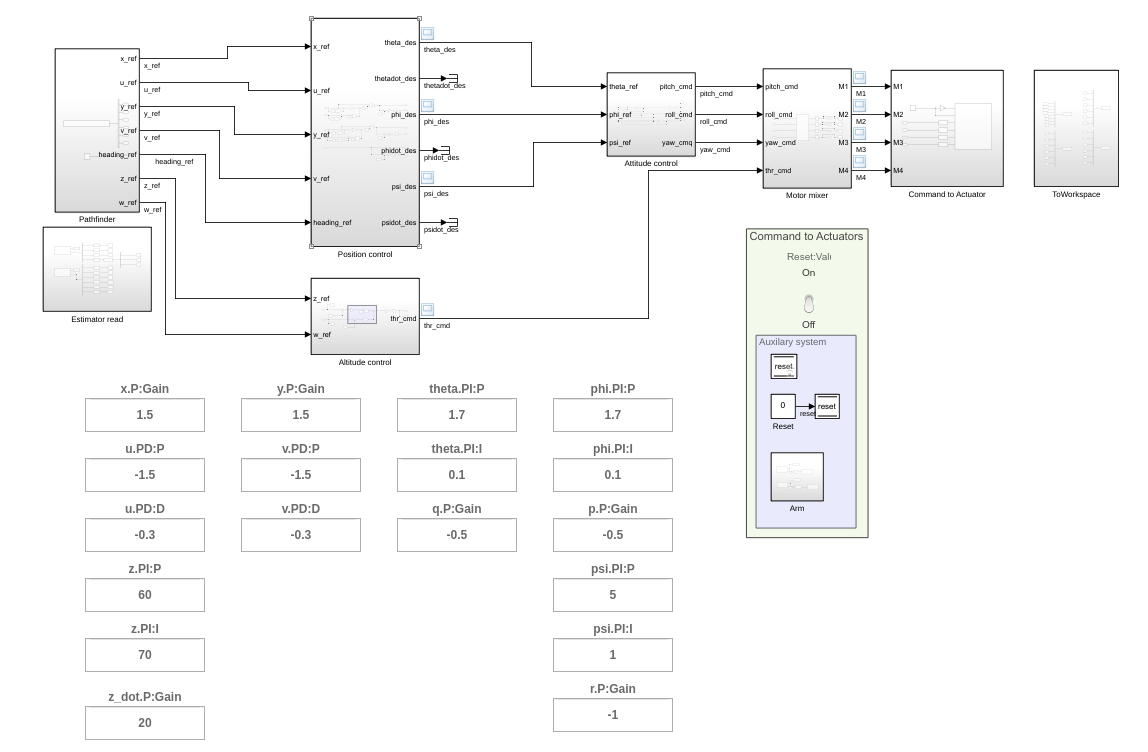
\includegraphics[width=1\textwidth]{DescrizioneAutopilota/Figure/completopid}
	\caption{Modello di controllo completo PID}
\end{figure}

\begin{figure}
	\centering
	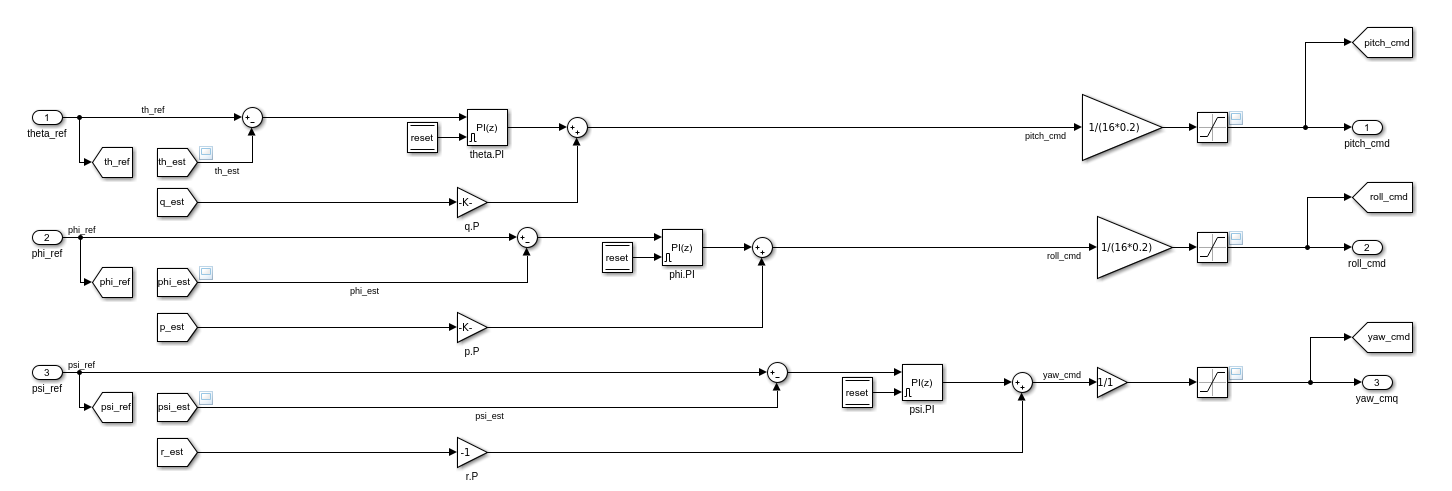
\includegraphics[width=1\textwidth]{DescrizioneAutopilota/Figure/attitudecontrollerpid}
	\caption{Modello di controllo d' assetto PID}
\end{figure}

\begin{figure}
	\centering
	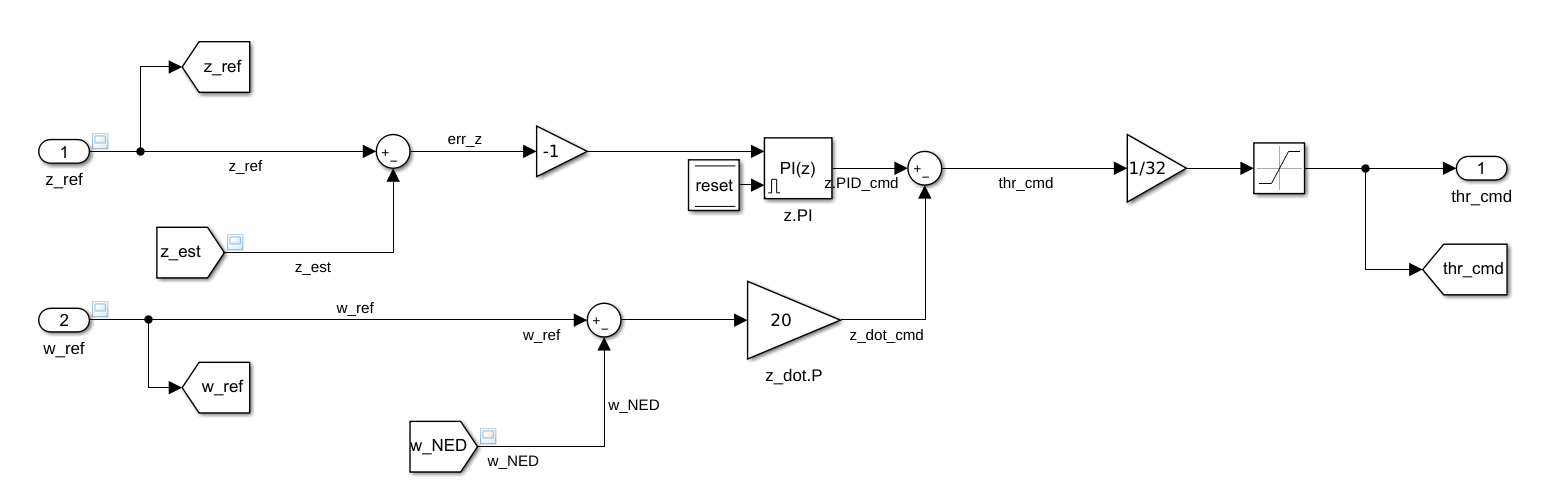
\includegraphics[width=1\textwidth]{DescrizioneAutopilota/Figure/altitudecontrollerpid}
	\caption{Modello di controllo di altitudine PID}
\end{figure}

\begin{figure}
	\centering
	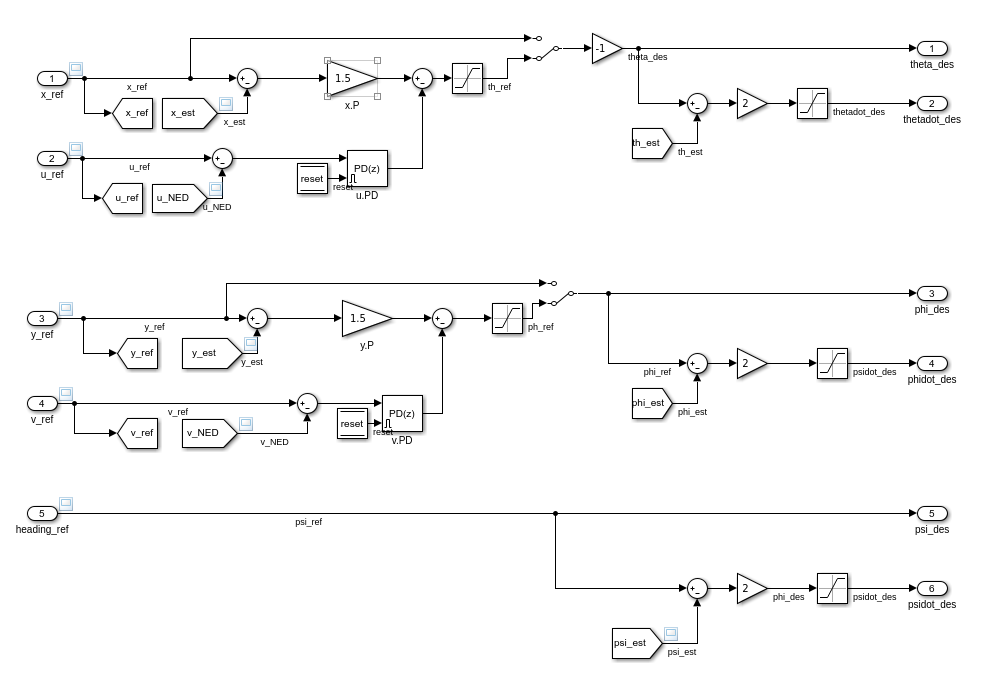
\includegraphics[width=1\textwidth]{DescrizioneAutopilota/Figure/positioncontrollerpid}
	\caption{Modello di controllo di posizione PID}
\end{figure}

\begin{figure}
	\centering
	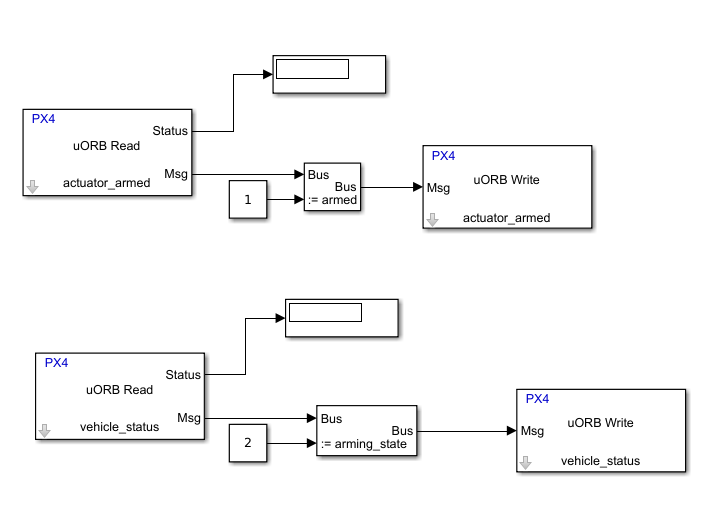
\includegraphics[width=0.5\textwidth]{DescrizioneAutopilota/Figure/armpid}
	\caption{Modello di gestione dei segnali di armamento}
\end{figure}